\chapter{Graphical User Interface}

Die graphische Benutzeroberfläche als Schnittstelle zwischen dem Nutzer und dem Simulatorkern soll den Anforderungen an eine moderne Anwendung gerecht werden und ein ansprechendes Design sowie hohe Benutzerfreundlichkeit als zentrale Merkmale implementieren. Dabei orientiert sich die Gestaltung an den Ansprüchen des Programms als Simulations- und Lernwerkzeug: Gute Verständlichkeit der dargestellten Inhalte, visuelle Hervorhebung technischer Zusammenhänge, sowie der Verzicht auf irreführende Vereinfachungen, wo dies möglich ist.


\section{Fenstermanagement}

Die graphische Benutzeroberfläche soll aus verschiedenen Modulen bestehen, die zunächst als Editor-, Register-, Speicher-, Snapshot-, Hilfs- und Output-Modul identifiziert wurden. Die darüberliegende Symbolleiste steuert Abläufe und Einstellungen, die über Modulgrenzen hinweg Relevanz haben.

Die Unterbringung der Module erfolgt in einem tabellarischen Layout bestehend aus 4 Spalten zu je 1 bis 2 Zeilen. Die untere Zeile einer Spalte kann je nach Bedarf angezeigt oder ausgeblendet werden.

Die dadurch entstehenden Modulzellen sollen variabel mit den oben beschriebenen Modulen belegt werden können, was die Möglichkeit mit einschließt, ein Modul mehrfach in verschiedenen Zellen anzuzeigen. Ein einfaches Anwendungsbeispiel für diese Funktionalität ist das parallele Arbeiten auf zwei Bereichen des Speichers.

\begin{figure}
  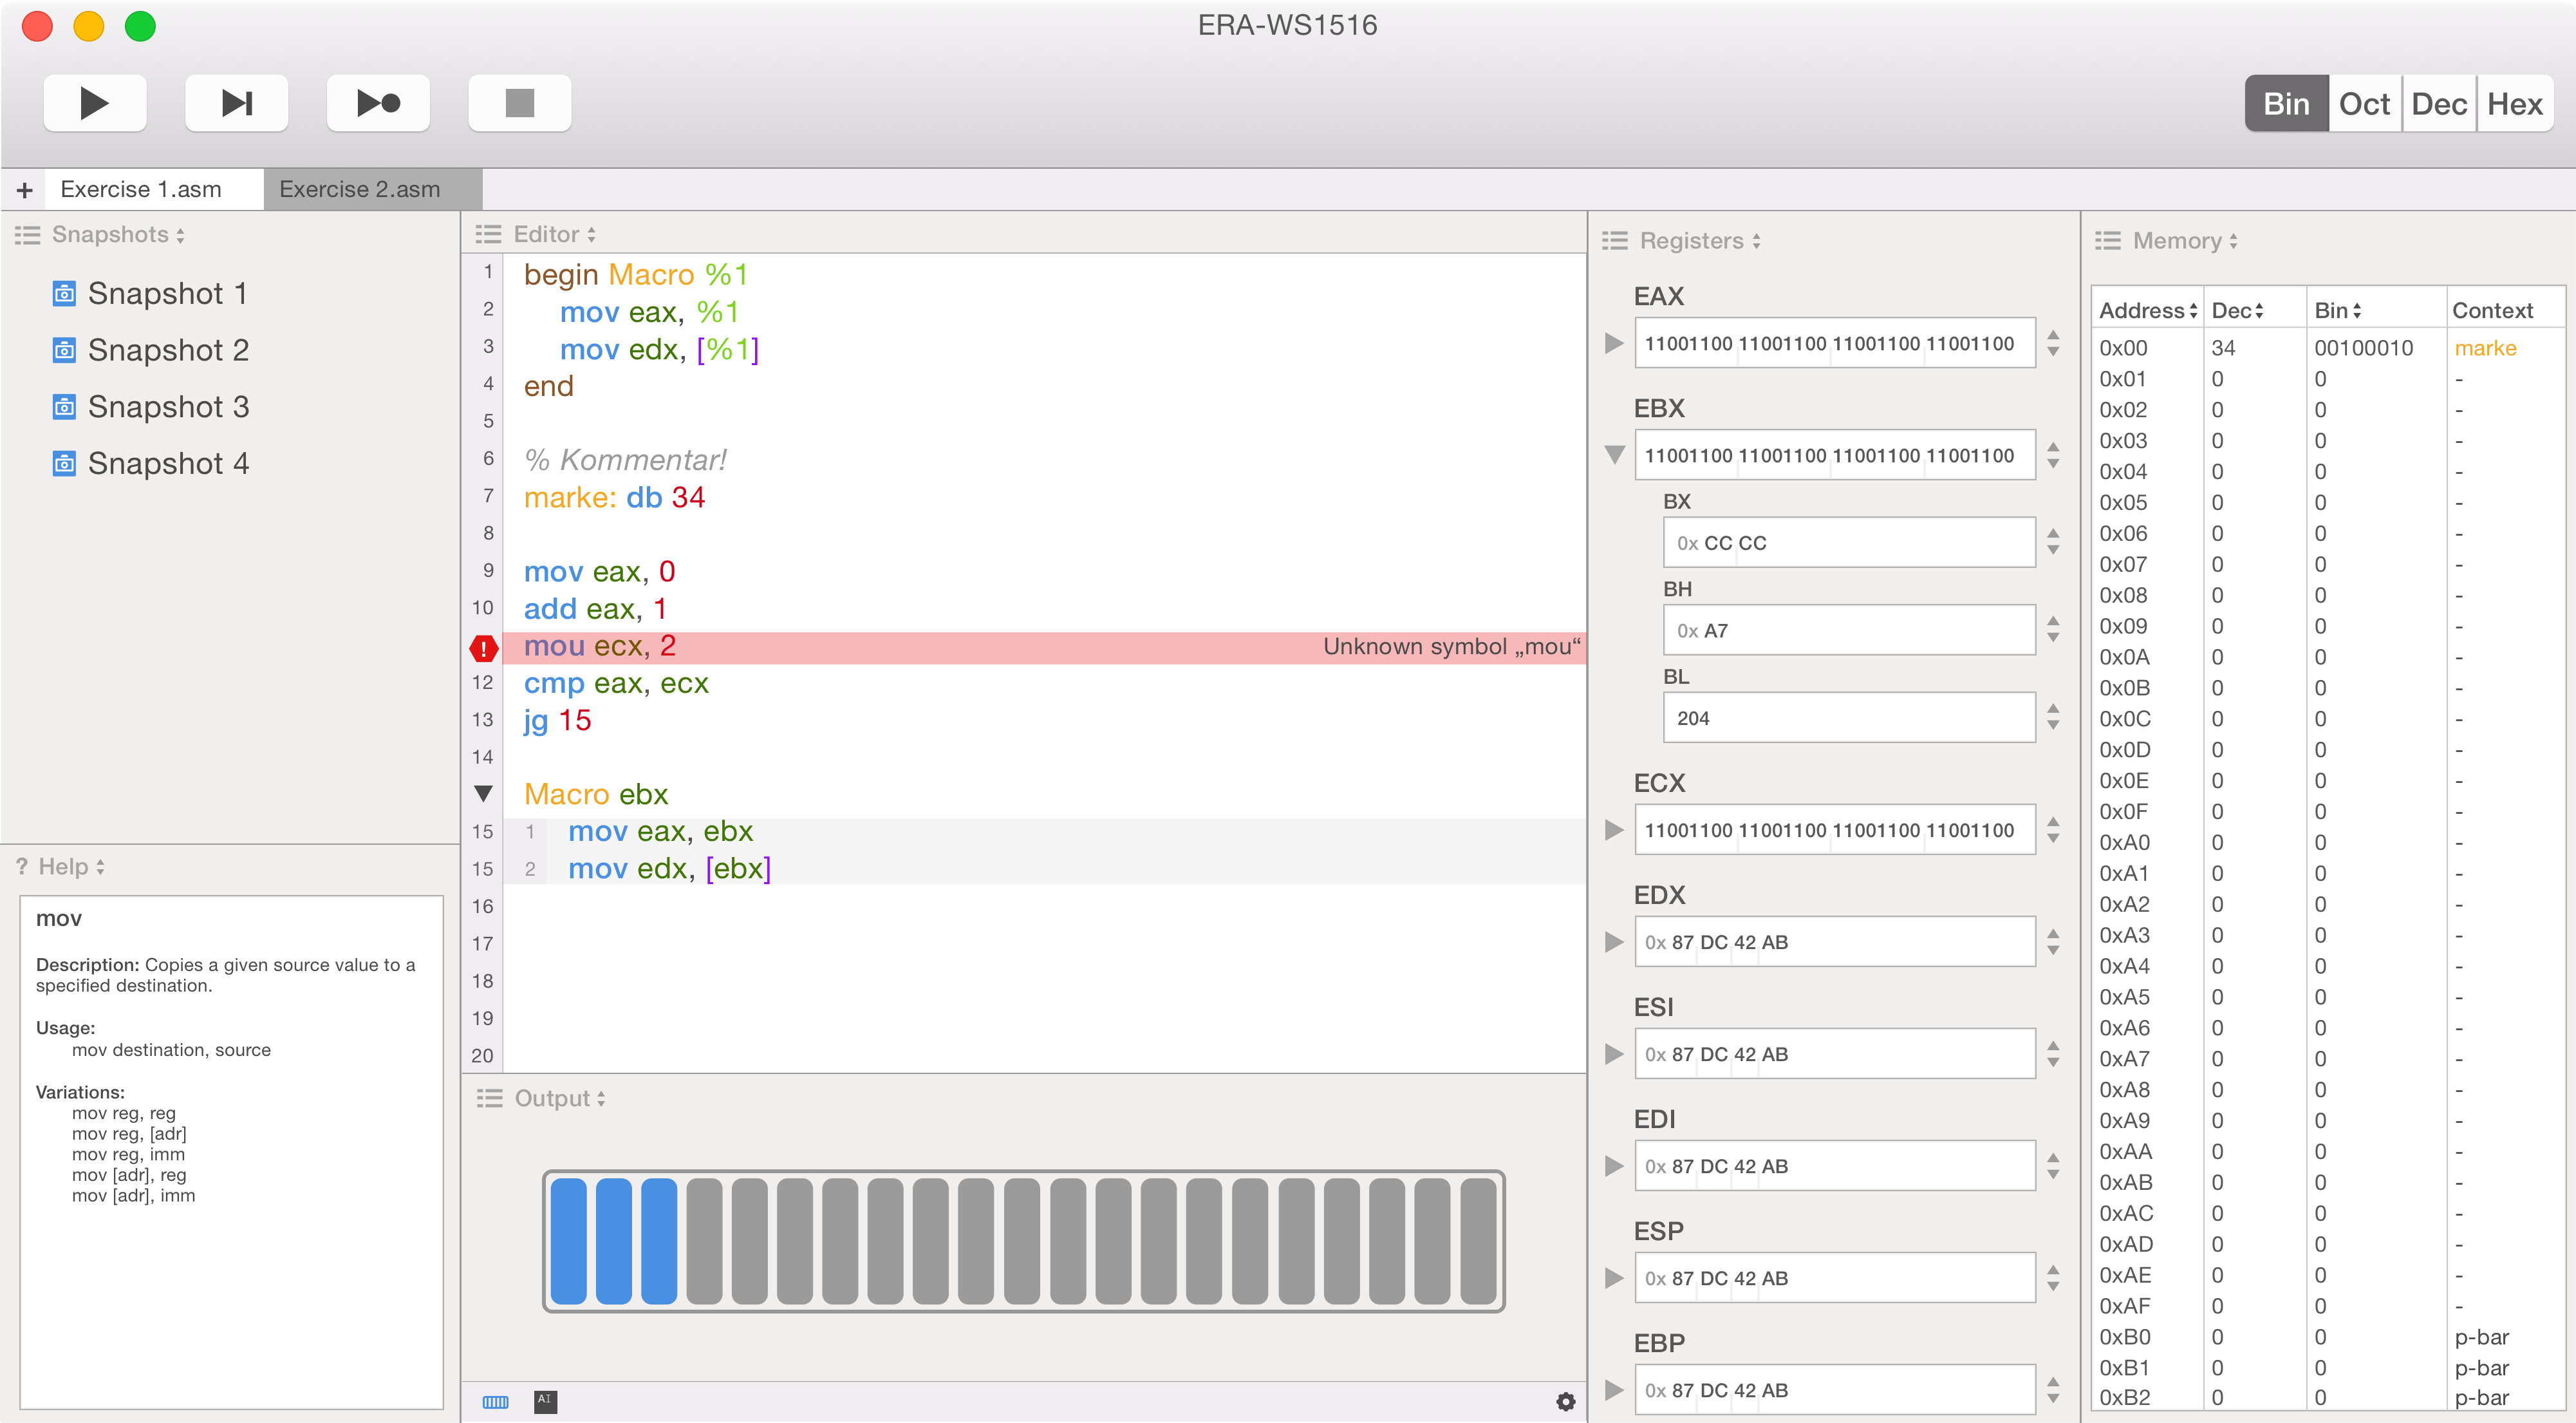
\includegraphics[width=\textwidth]{../ui/figures/mockup}
  \label{fig:Mockup}
  \caption{Der obige rein visuelle Entwurf soll einen groben Überblick über die geplante Umsetzung der Benutzeroberfläche geben. Im Wesentlichen ist die Aufteilung des Fensters in Symbolleiste und die vier Spalten mit ein bis zwei Zeilen erkennbar. Zudem wurden die einzelnen Module skizziert.}
\end{figure}

\subsection{Symbolleiste}

Über die Symbolleiste kann die Ausführung des Programms gesteuert werden, wobei die Optionen \textit{Ausführung des gesamten Programms}, \textit{Ausführung einer einzelnen Instruktion}, \textit{Ausführung bis zum
  nächsten Haltepunkt} und \textit{Abbrechen der Programmausführung} zur Verfügung stehen.

Des Weiteren lässt sich das Zahlenformat modulübergreifend festlegen, was insebesondere Einfluss auf Register- und Speicherinhalte hat.

\subsection{Editor}

Der Editor für die Eingabe der Assembler-Instruktion soll Syntax-Highlighting unterstützen, um Instruktions-Komponenten visuell zu trennen. Die Umsetzung erfolgt mit dem Qt-eigenen Syntax-Highlighter (\textit{QHighlighter}), welcher mit regulären Ausdrücken initialisiert wird. Diese werden vom Parser in Kombination mit Architektur-eigenen Schlüsselwörtern generiert und über den Core zur Verfügung gestellt.

Fehlermeldungen, die vom Parser ermittelt wurden, werden innerhalb der zugehörigen Zeile im Editor angezeigt. Dies ermöglich es, mehrere Fehlermeldungen gleichzeitig anzuzeigen.

Ein Makroaufruf wird im Editor als einzelne Zeile dargestellt, die bei Bedarf vom Benutzer aufgeklappt werden kann, wodurch die Makrodefinition an der selben Stelle eingeblendet wird. Dies ermöglicht u.a. die schrittweise Ausführung des Codes ohne Unterbrechungen oder Sprünge.

\subsection{Register}

Die Registerwerte werden übersichtlich mit Hilfe von Byte-Separatoren dargestellt. Zu den jeweiligen Registern gehörige Unterregister können separat eingeblendet werden.

Registern wie Unterregistern kann unabhängig von den globalen Einstellungen ein eigenes Zahlenformat (binär, hexadezimal etc.) zugewiesen werden.

Intern werden die einzelnen Zahlenformate vom Core berechnet und als String an das GUI-Modul übergeben.

\subsection{Speicher}

Der Speicher teilt sich in drei Hauptbereiche: Speicheradressen, Speicherinhalte und Kontextinformationen.
Der Adressraum erlaubt die Unterteilung in verschiedene Datenformate, darunter Byte, Halbwort, Wort etc.
Das Zahlenformat der Speicherinhalte ist spaltenweise anpassbar.

Kontextinformationen zu einzelnen Speicherzellen geben Hinweise auf die Verwendung im Programm, darunter etwa Marken zu Datendefinitionen, Speicherbereiche für Ausgabegeräte und Speicher-Referenzierungen durch Register.

Beim Assemblieren des Assembler-Codes werden die Instruktionen ins Binärformat übersetzt und in den Speicher geschrieben, um die technischen Grundlagen hinter der Ausführung eines Assemblerprogramms zu verdeutlichen. Die einzelnen Adresszellen werden mit den jeweils zugehörigen Zeilennummern in Form von Kontextinformation annotiert. Um zu verhindern, dass der Speicher aufgrund der vielen durch das assemblierte Programm besetzten Speicherzellen unübersichtlich wird, soll eine visuelle Trennung des Code-Bereichs vom Daten-Bereich vorgenommen werden.

\subsection{Snapshots}

Um schnell zwischen verschiedenen Register- und Speicherzuständen wechseln zu können, wird das Anelgen von sogenannten Snapshots unterstützt, in denen alle Register- und Speicherinhalte abgespeichert werden. Im Snapshot-Modul können die dem aktuellen Projekt zugeordneten Snapshots angezeigt und geladen werden.


\section{Implementierung}

Die GUI wird unter Verwendung des Qt-Frameworks implementiert, wobei hauptsächlich das Qt Quick-Modul zum Einsatz kommt, das die Erstellung der Benutzeroberfläche mit QML erlaubt. Dessen Einsatz wiederum begünstigt die strikte Trennung des Models, das in Gestalt des Cores und der dahinterliegenden Module in C++ implementiert ist, vom View, dessen Umsetzung im Wesentlichen in QML und JavaScript erfolgt.

\subsection{View}

Die Modularität der Benutzeroberfläche spiegelt sich auch in der strukturellen Entwurf der GUI-Module in QML wieder, wo diese durch die jeweils eigenständigen Komponenten implementiert sind.

\subsection{Model-View-Schnittstelle}

Der Core kann über das Observer-Entwurfsmuster mit dem View kommunizieren und benötigt somit keine Information über die interne Struktur des Views.

Die Kommunikation in umgekehrter Richtung, also der Zugriff des Views auf die Daten des Models, basiert auf dem von QML unterstützten Muster, das den Datenaustausch über Delegates regelt. Damit nach diesem Muster ausgehend von QML-Objekten auf Daten des Models zugegriffen werden kann, wird eine C++-Schnittstelle bestehend aus \textit{QObject}-Klassen benötigt, die zwischen beiden Modulen vermittelt.
